%\documentclass[12pt,fullpage,doublespace]{elsart}
\documentclass[10pt,twocolumn]{elsart5p}
\usepackage{graphicx}
\usepackage{dcolumn}
\usepackage{amsmath}
\usepackage{amssymb}
\usepackage{bm}
\usepackage{natbib}


\begin{document}

\begin{frontmatter}

\title{SPIKY:A graphical user interface for monitoring spike train synchrony}

\author{Thomas Kreuz},
\ead{thomas.kreuz@cnr.it}
\author{Nebojsa Bozanik}
%\author[ITT]{Daniel Chicharro},
%\author[UBE]{Conor Houghton},
%\author[UPF]{Ralph G. Andrzejak},
%\author[UBG]{Florian Mormann}

\address[ISC]{Institute for complex systems, CNR, Sesto Fiorentino, Italy}
%\address[ITT]{Center for Neuroscience and Cognitive Systems@UniTn, Italian Institute of Technology, Rovereto (TN), Italy}
%\address[UBE]{Department of Computer Science, University of Bristol, Bristol, England}
%\address[UPF]{Department of Information and Communication Technologies, Universitat Pompeu Fabra, Barcelona, Spain}
%\address[UBG]{Department of Epileptology, University of Bonn, Bonn, Germany}


\date{\today}

\begin{abstract}
    Recently, the SPIKE-distance has been proposed as a measure of spike train synchrony which is both parameter-free and time-scale independent. Since it relies on instantaneous estimates of spike train dissimilarity, it is also time-resolved which makes it possible to track changes in instantaneous clustering, i.e., time-localized patterns of (dis)similarity among multiple spike trains. Further features include selective and triggered temporal averaging as well as the instantaneous comparison of spike train groups. Besides the regular SPIKE-distance, there also exists a causal variant which is defined such that the instantaneous values of dissimilarity rely on past information only so that time-resolved spike train synchrony can be estimated in real-time. Finally, here we introduce the future SPIKE-distance which can be used in triggered temporal averaging in order to evaluate the effect of certain spikes or of certain stimuli features on future spiking. In the first part of this report we address some of the computational aspects in the calculation and implementation of the SPIKE-distance while in the second part we present SPIKY, a graphical user interface which facilitates the application of the SPIKE-distance and all its variants to both simulated and real data.
\end{abstract}


\begin{keyword}
    time series analysis; spike trains; clustering; neuronal coding
\end{keyword}

\end{frontmatter}

\newcommand{\abb}{\small\sf}

%
% ********************************************************************************************** Intro **************
%
\section{\label{s:Intro} Introduction}

A wide variety of approaches to quantify the dissimilarity, or distance, between two spike trains has been suggested. Among these is the metric introduced in \citet{Victor96},
which evaluates the cost needed to transform one spike train into the other, using only certain elementary steps. Another metric proposed in \citet{VanRossum01}, measures the
Euclidean distance between the two spike trains after convolution of the spikes with an exponential function. Both methods involve one parameter that sets the time scale. In
contrast, two more recent bivariate approaches, the ISI- and the SPIKE-distance are time scale independent and self-adaptive \citep{Kreuz07c, Kreuz12a}. These two measures are complementary: The ISI-distance relies on the relative length of simultaneous interspike intervals and is thus well-designed to quantify similarities in the neurons� firing-rate profiles \citep{Kreuz07c, Kreuz09}. The SPIKE-distance is based on differences between the spike times of the two spike trains and is therefore ideally suited to track synchrony that is mediated by spike timing \citep{Kreuz11, Kreuz12a}.

XXXXX Computational aspects XXXXX

%
% ********************************************************************************************** Methods **************
%
\section{\label{s:Methods} Methods}

XXXXX maybe shift definition of distances to the appendix XXXXX



\section{\label{ss:SPIKE-Distance} The SPIKE-distance}

The SPIKE-distance (see \citet{Kreuz11} for the original proposal and \citet{Kreuz12a} for the definite version presented here) is extracted from differences between the spike times of the two spike trains. It relies on instantaneous values in the sense that in a first step the two sequences of discrete spike times are transformed into a continuous dissimilarity profiles $S (t)$. This dissimilarity profile is based on three piecewise constant quantities which for each neuron $n = 1, 2$ are assigned to every time instant between $0$ and $T$ (see Fig. \ref{fig:App-Fig1-SPIKE-Illustration}). These are the time of the preceding spike
%
\begin{equation} \label{eq:Prev-Spike}
    t_{\mathrm {P}}^x (t) = \max(t_i^n | t_i^n \leq t)  \quad t_1^n \leq t \leq t_{M_n}^n,
\end{equation}
%
the time of the following spike
%
\begin{equation} \label{eq:Foll-Spike}
    t_{\mathrm {F}}^n (t) = \min(t_i^n | t_i^n > t)  \quad t_1^n \leq t \leq t_{M_n}^n,
\end{equation}
%
as well as the interspike interval
%
\begin{equation} \label{eq:ISI}
    x_{\mathrm {ISI}}^n (t) = t_{\mathrm {F}}^n (t) - t_{\mathrm {P}}^n (t).
\end{equation}
%
The ambiguity regarding the definition of the very first and the very last interspike interval is resolved by placing for each spike train auxiliary leading spikes at time $t = 0$ and auxiliary trailing spikes at time $t = T$.
%
\begin{figure}
    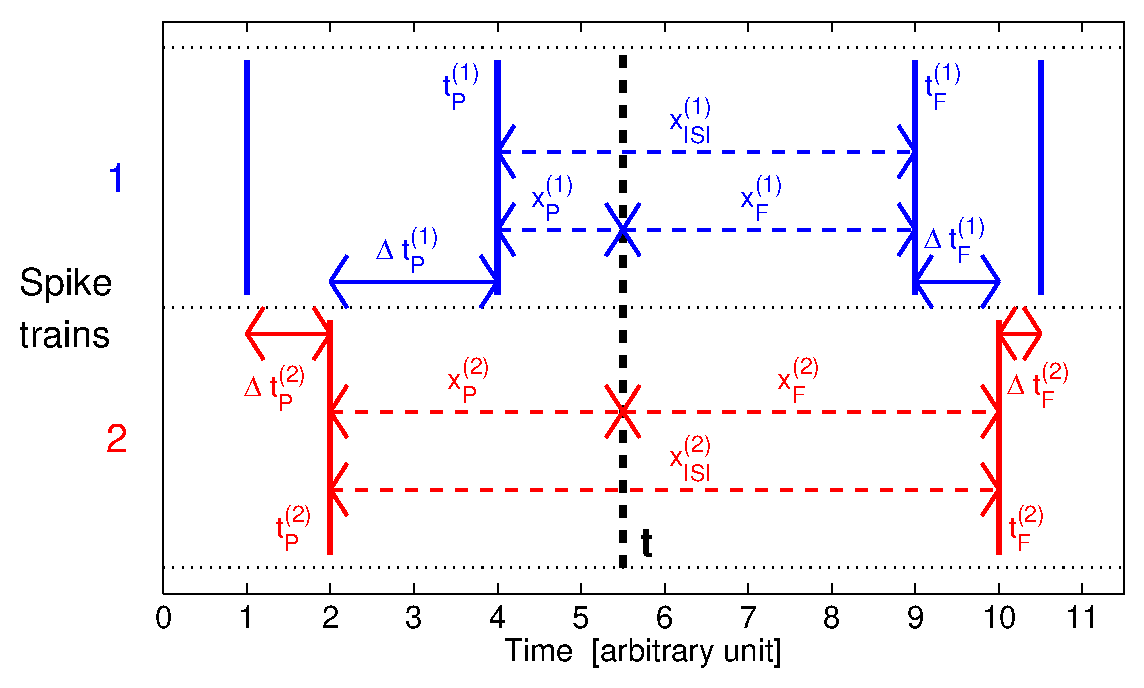
\includegraphics[width=85mm]{Fig1_SPIKE_Illustration.eps}
    \caption{\abb\label{fig:Fig1-SPIKE-Illustration} SPIKE-distance. Illustration of the local quantities needed to define the dissimilarity profile $S (t)$ for an arbitrary time instant $t$.}
\end{figure}
%
From these three quantities the dissimilarity profile is calculated in two steps: First for each spike the distance to the nearest spike in the other spike train is calculated, then for each time instant the relevant spike time differences are selected, weighted, and normalized. Here �relevant� means local; each time instant is uniquely surrounded by four corner spikes: the preceding spike from the first spike train $t_{\mathrm {P}}^{(1)}$, the following spike from the first spike train $t_{\mathrm {F}}^{(1)}$, the preceding spike from the second spike train $t_{\mathrm {P}}^{(2)}$, and, finally, the following spike from the second spike train $t_{\mathrm {F}}^{(2)}$. Each of these corner spikes can be identified with a spike time difference, for example, for the previous spike of the first spike train
%
\begin{equation} \label{eq:Delta-Corner-Spike}
     \Delta t_{\mathrm {P}}^{(1)} = \min_i (| t_{\mathrm {P}}^{(1)} - t_i^{(2)} |)
\end{equation}
%
and analogously for $t_{\mathrm {F}}^{(1)}$, $t_{\mathrm {P}}^{(2)}$, and $t_{\mathrm {F}}^{(2)}$  (see Fig. \ref{fig:App-Fig1-SPIKE-Illustration}). For each spike train separately a locally weighted average is employed such that the differences for the closer spike dominate; the weighting factors depend on
%
\begin{equation} \label{eq:Prev-Spike-Dist}
     x_{\mathrm {P}}^{(n)} (t) = t - t_{\mathrm {P}}^{(n)} (t)
\end{equation}
%
and
%
\begin{equation} \label{eq:Foll-Spike-Dist}
     x_{\mathrm {F}}^{(n)} (t) = t_{\mathrm {F}}^{(n)} (t) - t,
\end{equation}
%
the intervals to the previous and the following spikes for each neuron $n = 1, 2$. The local weighting for the spike time differences of the first spike train reads
%
\begin{equation} \label{eq:Bi-Spike-Diss-Improved-First}
     S_1 (t) = \frac{\Delta t_{\mathrm {P}}^{(1)} x_{\mathrm {F}}^{(1)} + \Delta t_{\mathrm {F}}^{(1)} x_{\mathrm {P}}^{(1)}}{x_{\mathrm {ISI}}^{(1)}}
\end{equation}
%
and analogously $S_2 (t)$ is obtained for the second spike train. Averaging over the two spike train contributions and normalizing by the mean interspike interval yields
%
\begin{equation} \label{eq:Bi-Spike-Diss-Improved-Intermediate}
     S'' (t) = \frac{S_1 (t) + S_2 (t)}{2 \langle x_{\mathrm {ISI}}^{(n)} \rangle_n}.
\end{equation}

This quantity weights the spike time differences for each spike train according to the relative distance of the corner spike from the time instant under investigation. This way relative distances within each spike train are taken care of, while relative distances between spike trains are not. In order to get these ratios straight and to account for differences in firing rate, in a last step the two contributions from the two spike trains are locally weighted by their instantaneous interspike intervals. This leads to the improved definition of the dissimilarity profile
%
\begin{equation} \label{eq:Bi-Spike-Diss-Improved}
     S (t) = \frac{S_1 (t) x_{\mathrm {ISI}}^{(2)} + S_2 (t) x_{\mathrm {ISI}}^{(1)}}{2 \langle x_{\mathrm {ISI}}^{(n)} \rangle_n^2}.
\end{equation}

The SPIKE-distance is defined as the temporal average of this dissimilarity profile
%
\begin{equation} \label{eq:Bi-Spike-Distances}
    D_S = \frac{1}{T} \int_{t=0}^T dt S (t).
\end{equation}
%
The dissimilarity profile $S (t)$ and the SPIKE-distance $D_S$ as its average are bounded in the interval $[0, 1]$. The distance value $D_S = 0$ is obtained for identical spike trains only.

There exists a straightforward extension to the case of more than two spike trains (number of spike trains $N > 2$), the averaged bivariate distance. This average over all pairs of neurons commutes with the average over time, so it is possible to achieve the same kind of time-resolved visualization as in the bivariate case by first calculating the instantaneous average, e.g., $S^{\mathrm {a}} (t)$ over all pairwise instantaneous values $S^{mn} (t)$,
%
\begin{equation} \label{eq:Bivariate-Average}
    S^{\mathrm {a}} (t) = \frac{1}{N(N-1)/2}\sum_{n=1}^{N-1} \sum_{m=n+1}^N S^{mn} (t)
\end{equation}

The Matlab source code for calculating and visualizing the SPIKE-distance can be found under http://www.fi.isc. cnr.it/users/thomas.kreuz/sourcecode.html.


\subsection{\label{ss:Real-time-Spike-Distance} Realtime SPIKE-distance}

The Realtime SPIKE-distance $D_{S_r}$ is a modification of the SPIKE-distance with the key difference that the corresponding
time profile $S_r(t)$ can be calculated online because it relies on past information only. From the perspective of an online measure, the information provided by the following spikes, both their position and the length of the interspike interval, is not yet available. Like the regular (improved) SPIKE-distance $D_S$, this causal variant is also based on local spike time differences but now only two corner spikes are available, and the spikes of comparison are restricted to past spikes, e.g., for the preceding spike of the first spike train
%
\begin{equation} \label{eq:Delta-Corner-Spike-Realtime}
     \Delta t_{\mathrm {P}}^{(1)} = \min_i (| t_{\mathrm {P}}^{(1)} - t_i^{(2)} |), t_i < t.
\end{equation}
%
Since there are no following spikes available, there is no local weighting, and since there is no interspike interval, the normalization is achieved by dividing the average corner spike difference by twice the average time interval to the preceding spikes (Eq. \ref{eq:Prev-Spike-Dist}). This yields a causal indicator of local spike train dissimilarity:
%
\begin{equation} \label{eq:Bi-Spike-Diss-RT}
    S_r (t) = \frac{ \Delta t_{\mathrm {P}}^{(1)} + \Delta t_{\mathrm {P}}^{(2)}} {4 \langle x_{\mathrm {P}}^{(n)} \rangle_n}.
\end{equation}

\subsection{\label{ss:Future-Spike-Distance} Future SPIKE-distance}

The future SPIKE-distance $D_{S_f}$ can be used in triggered temporal averaging in order to evaluate the effect of certain spikes or of certain stimuli features on future spiking. It is the inverse measure to the Realtime SPIKE-distance but instead of relying on past information only it relies on future information only. Also in this case for each time instant just two corner spikes are available, since the spikes of comparison are restricted to future spikes only. Thus the spike time difference for the following spike of the first spike train reads
%
\begin{equation} \label{eq:Delta-Corner-Spike-Future}
     \Delta t_{\mathrm {F}}^{(1)} = \min_i (| t_{\mathrm {F}}^{(1)} - t_i^{(2)} |), t_i > t,
\end{equation}
%
and accordingly for the following spike of the second spike train. And, similar to Eq. \ref{eq:Bi-Spike-Diss-RT}, an indicator of local spike train dissimilarity is obtained as follows:
%
\begin{equation} \label{eq:Bi-Spike-Diss-FT}
    S_f (t) = \frac{ \Delta t_{\mathrm {F}}^{(1)} + \Delta t_{\mathrm {F}}^{(2)}} {4 \langle x_{\mathrm {F}}^{(n)} \rangle_n}.
\end{equation}


\subsection{\label{ss:Bivariate-ISI-Distance} The ISI-distance}

While the dissimilarity profile of the SPIKE-distance is extracted from differences between the spike times of the two spike trains, the dissimilarity profile of the ISI-distance \citep{Kreuz07c, Kreuz09} is calculated as the instantaneous ratio between the interspike intervals $x_{\mathrm {ISI}}^{(1)}$ and $x_{\mathrm {ISI}}^{(2)}$ (Eq. \ref{eq:ISI}) according to:
%
\begin{equation} \label{eq:ISI-Ratio}
    I (t) = \begin{cases}
           x_{\mathrm {ISI}}^{(1)} (t) / x_{\mathrm {ISI}}^{(2)} (t) - 1 & {\rm if} ~~ x_{\mathrm {ISI}}^{(1)} (t) \leq x_{\mathrm {ISI}}^{(2)} (t) \cr
                      - (x_{\mathrm {ISI}}^{(2)} (t) / x_{\mathrm {ISI}}^{(1)} (t) -1)     & {\rm otherwise}.
                  \end{cases}
\end{equation}
%
This ISI-ratio equals $0$ for identical ISI in the two spike trains, and approaches $-1$ and $1$, respectively, if the first or the second spike train is much faster than the other. For the ISI-distance the temporal averaging analogous to Eq. \ref{eq:Temporal-Average} is performed on the absolute value of the ISI-ratio, thus both kinds of deviations are treated equally. Since the ISI-distance relies on the instantaneous ISI-values and thus requires knowledge about the following spikes, no causal Realtime extension is possible.


\section{\label{s:Results} Results}

\subsection{\label{ss:Computational-aspects} Computational aspects}

XXXXX Rewrite and extend, add part on MEX-files XXXXX

The improved dissimilarity profile $S (t)$ of the SPIKE-distance is piecewise linear (with each linear interval running
from one spike of the pooled spike train to the next) rather than piecewise constant as is the case for the ISI-distance.
Therefore, when the localized visualization is desired, a new value has to be calculated for each sampling

point and not just once per each interval in the pooled spike train. In cases where the distance value itself is sufficient,
the short computation time can be even further decreased by representing each interval by the value of its center and
weighting it by its length. This is not only faster, but it actually gives the exact result, whereas the time-resolved calculation is a very good approximation only for sufficiently small sampling intervals dt (imagine the example of a rectangular
function, at some point any sampled representation has to cut the right angle). The dissimilarity profiles $S_r(t)$
and $S_f (t)$ of the real-time and the future SPIKE-distances are hyperbolic and not linear but here also the exact result
can be obtained by piecewise integration over all intervals of the pooled spike train.
XXXXX Add figure on Pico vs. sampled XXXXX

The calculation of the SPIKE-distance consists of three steps: In a precalculation step, for each spike the distance to
the nearest spike in all the other spike trains is calculated. Successively, for each time instant and each pair of spike
trains, the distances of the four corner spikes are first locally weighted and then normalized. These latter steps involve
matrices of the order �number of time instants� � �number of spike train pairs�, which for very long datasets with many
spike trains can lead to memory problems. The solution to these problems is to make the calculation sequential, i.e.,
to cut the recording interval into smaller segments, and to perform the averaging over all pairs of spike trains for
each segment separately (no additional auxiliary spikes are needed except for very huge datasets for which even the calculation
of the first matrix is too memory-demanding). In the end the dissimilarity profiles for the different segments (already averaged over pairs of spike trains) are concatenated, and its temporal average yields the distance value for the whole recording interval.

The computational load scales with the number of spike trains $N$ as $N^2$. More information on the implementation as well as the Matlab source code for both the ISI- and the SPIKE-distance (including its real-time variant) can be found at www.fi.isc.cnr.it/users/thomas.kreuz/sourcecode.html.


\subsection{\label{ss:SPIKY} SPIKY}

XXXXXXXXXX


\section{\label{s:Discussion} Discussion}


\begin{appendix} \label{Appendix}

\end{appendix}


\vspace{1cm}

\begin{thanks}
\section{\label{s:Acknowledgement} \textbf{Acknowledgements}}
     TK acknowledges funding support from the European Commission through the Marie Curie Initial Training Network 'Neural Engineering Transformative Technologies (NETT)', project 289146 as well as from the Italian Ministry of Foreign Affairs regarding the activity of the Joint Italian-Israeli Laboratory on Neuroscience.
\end{thanks}


\bibliography{Literaturliste}

%\bibliographystyle{plainnat}
\bibliographystyle{elsart-harv}

\end{document}
